\chapter{Description of experiments}
\label{sec:experiments}
\section{Measure acceptance angle}
As a general verification of the system and a second verify the
alignment of the MMA on the back focal plane of the objective lens, we
imaged three fluorescent plane samples with various embedding indices.

The illumination in the sample was set to a disk of $\unit[30]{\mu m}$
diameter, spanning nearly the full field. Then a window of
$15\times15$ pixels was scanned over the MMA (6\% of BFP diameter) and
for each position, a camera image was
captured. \figref{fig:immersion-bfp-scan} displays the integrated
intensity in each image for each of the positions on the back focal
plane.

The left diagram shows an image of the pupil of the objective. Rays in
the edges of the MMA are absorbed by the pupil aperture in the
objective and therefore dark. The next two images show the reduced
acceptance angle due to lower index embedding medium. Rays on the
border of the pupil traverse the objective but are reflected at the
coverslip--embedding interface.

\begin{figure}[H]
  \centering
  \input{tirf-exp.eps_tex} 
  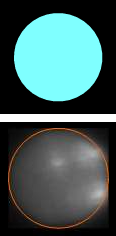
\includegraphics[height=69.56mm]{screen_mma-disk-integrate_rot}
  \caption{A fluorescent plane on a slide is embedded in oil, water or
    air. The thickness of the embedding medium is approximately
    $\unit[5]{\mu m}$. The LCoS illuminates a disk with $\unit[30]{\mu
      m}$ diameter while a $15\times 15$ window is scanned over the
    MMA. The window corresponds to a square with $\unit[210]{\mu m}$ on the side as opposed to \unit[3.6]{mm} BFP diameter {\bf right top:} LCoS mask. {\bf right bottom:} Typical
% 200 px diameter on LCoS
% 15x15 px full diameter is D=2*(R=f*NA) f=164.5/63=2.61  NA=1.38
% D=3.6mm -> D/256*15 = 210 um
    camera image.}
  \label{fig:tirf-exp}
\end{figure}


\begin{figure}[H]
  \centering
  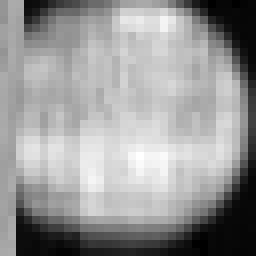
\includegraphics[width=4cm]{oil}
  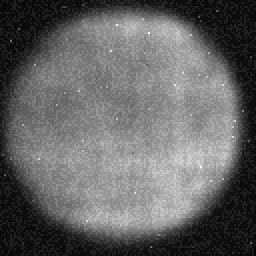
\includegraphics[width=4cm]{water}
  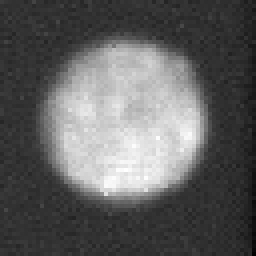
\includegraphics[width=4cm]{air}
  \caption{Integrated image intensities for different illumination
    window positions in the back focal plane. Embedding media: {\bf
      left:} Oil $n=1.52$, {\bf middle:} water $n=1.33$, {\bf right:}
    air $n=1$.  }
  \label{fig:immersion-bfp-scan}
\end{figure}

\section{Spatio-angular illumination of beads}
Here we describe the experiment that generated the data in
\figref{fig:bfp2-bfp-images-and-model}. The system configuration is
described in Appendix~\ref{sec:dvi_slow}. The LCoS controller was
connected to the graphics card. The camera exposure was fixed to
\unit[16]{ms}. The MMA mirrors were deflected during the integration
time. Between image changes on LCoS and MMA the system was paused for
several frames in order to prevent exposures with the wrong MMA or
LCoS masks (see \figref{fig:dvi-mosaic}).

\figref{fig:m_wf} shows slices of a wide field stack of a
three-dimensional distribution of $\unit[2]{\mu m}$ yellow-green beads
in Agar. The distance between the slices is $\unit[1]{\mu m}$. For
this acquisition both LCoS and MMA showed white patterns. The full
back focal plane was illuminated and the field of view in the sample
is a circle of \unit[25]{$\mu$m}.

\begin{figure}[H]
  \centering
  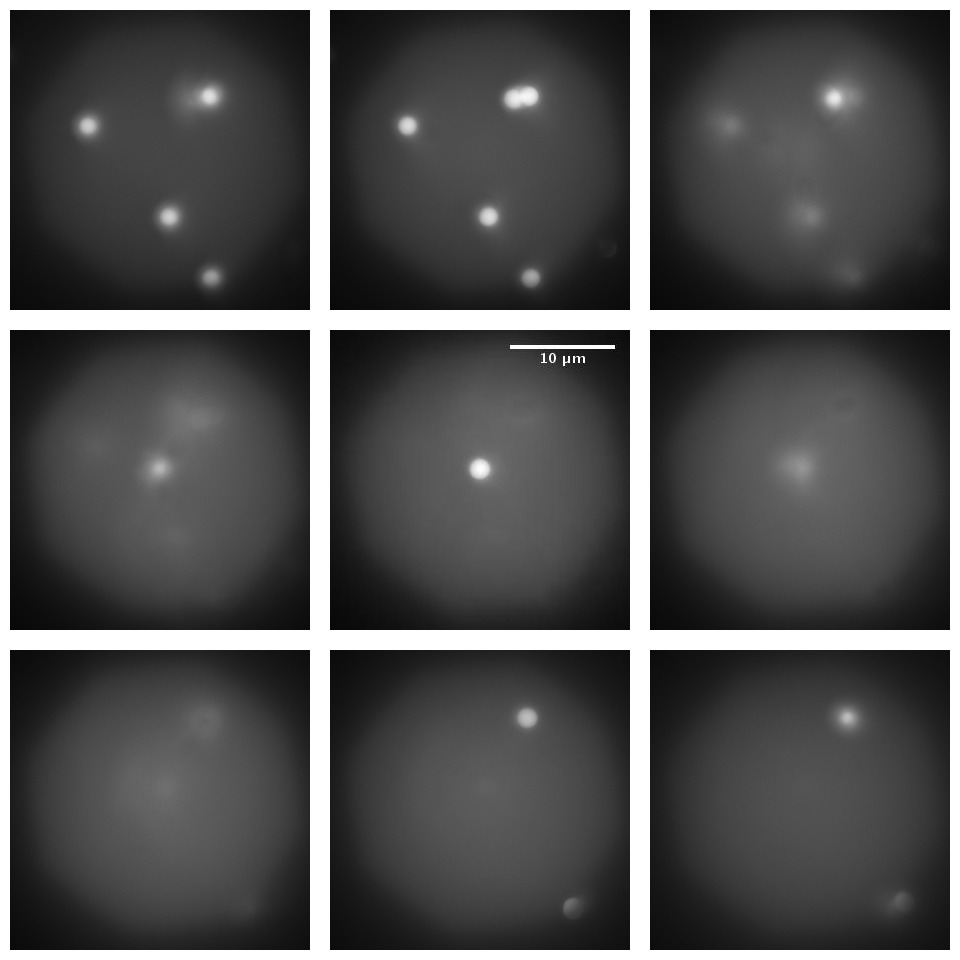
\includegraphics[width=12cm]{m_wf}
  \caption{Wide field stack of a three-dimensional distribution of
    yellow-green beads in agar. Sampling in $z$ is $\unit[1]{\mu m}$.}
  \label{fig:m_wf}
\end{figure}

\begin{figure}[H]
  \centering
  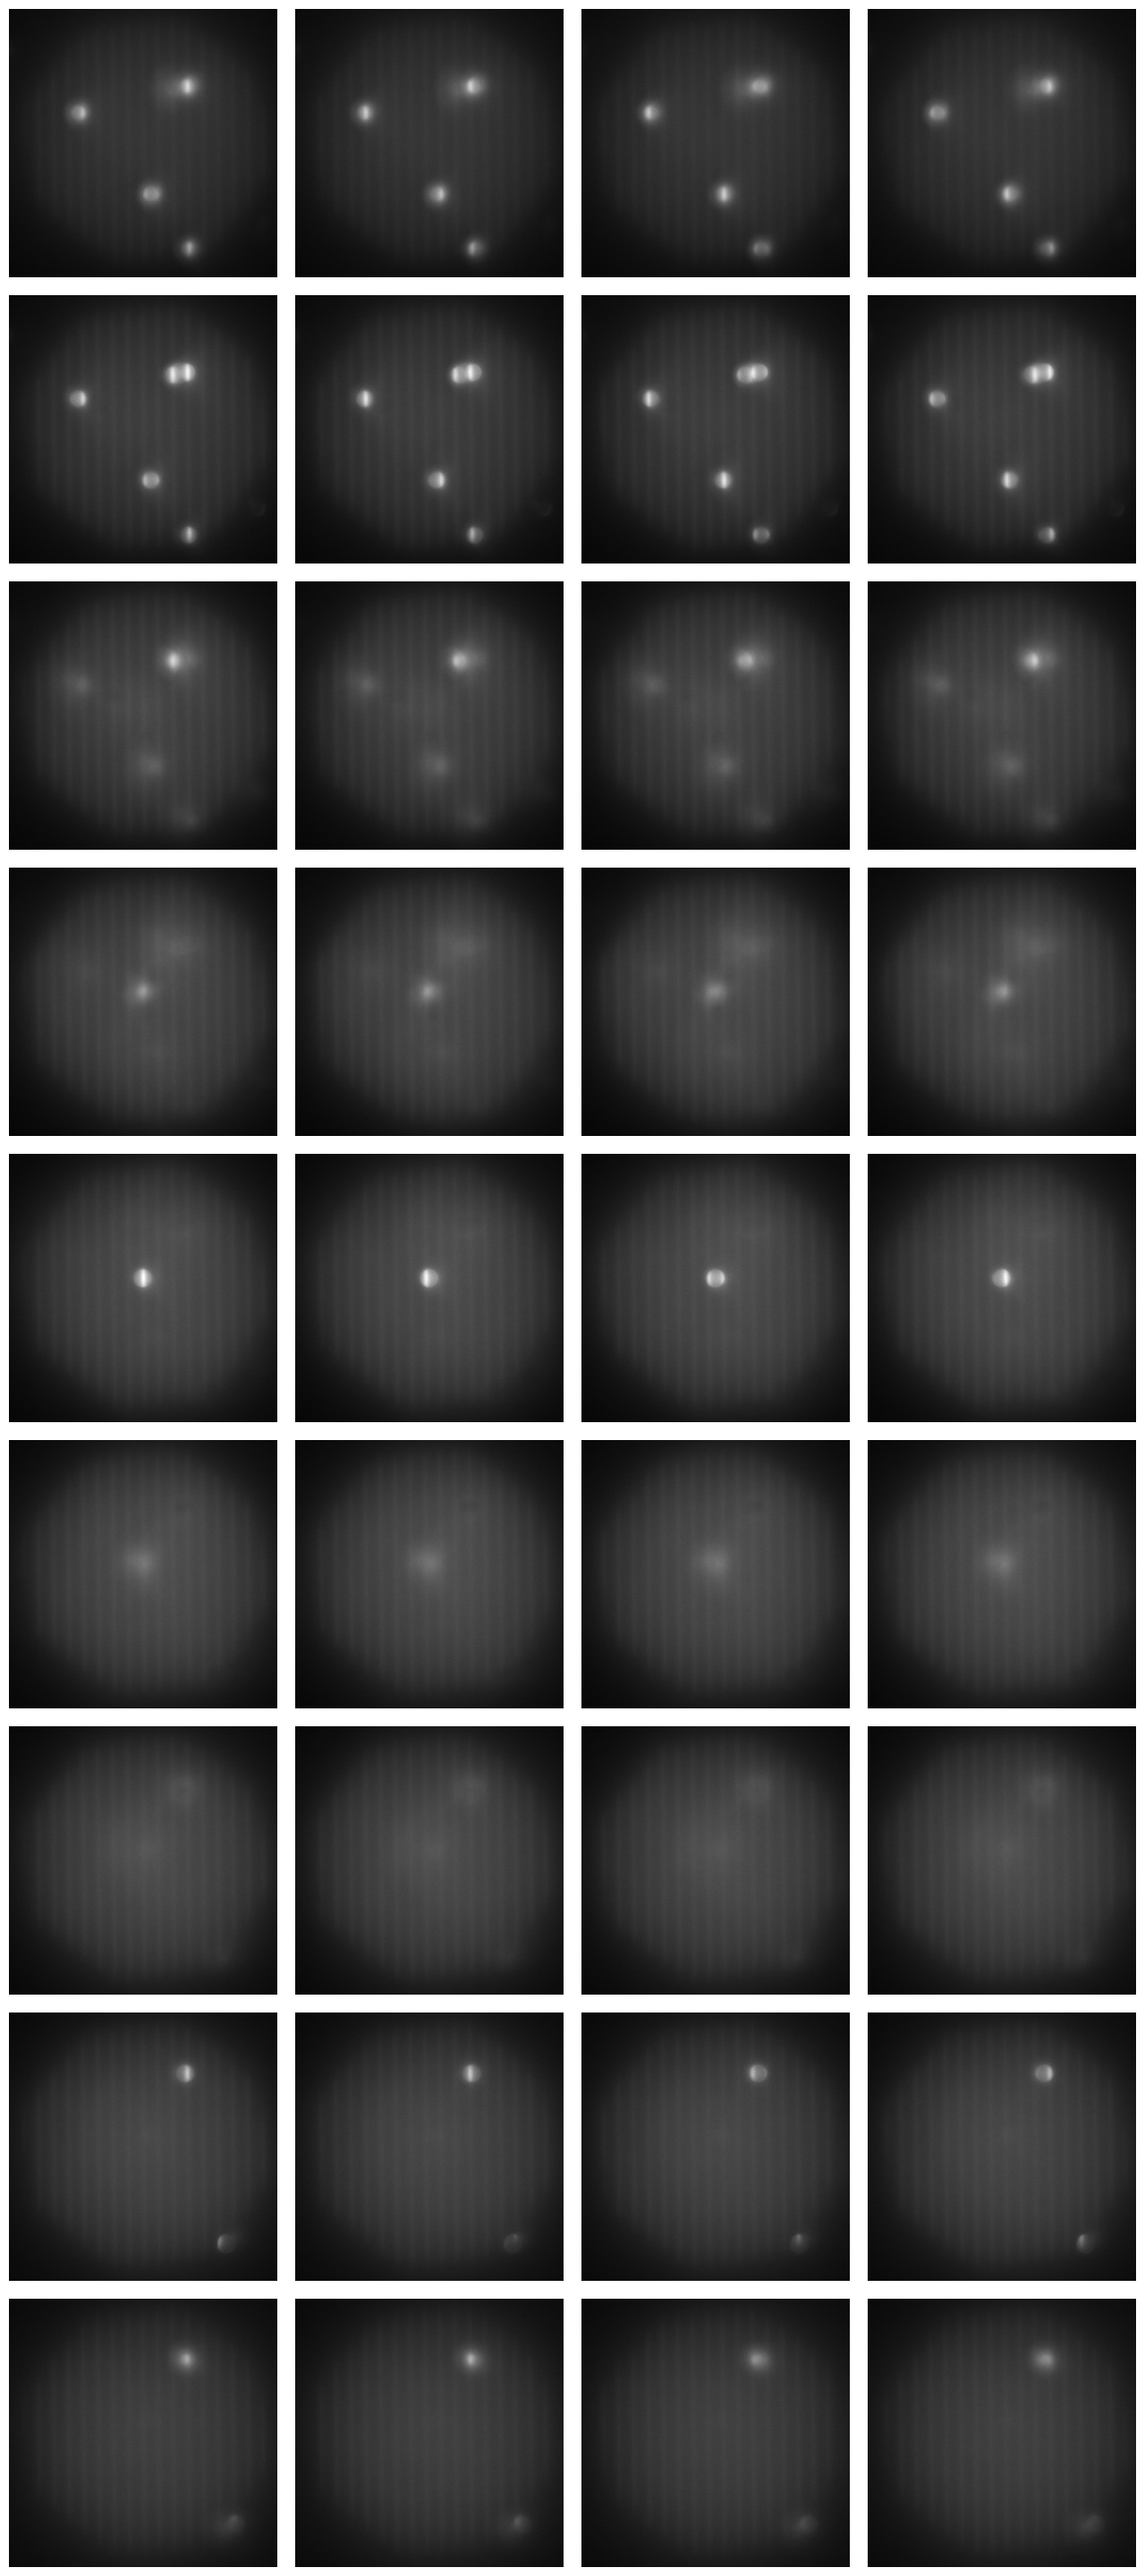
\includegraphics[height=.9\textheight]{m_phase}
  \caption{Structured illumination images of the same of the beads
    from \figref{fig:m_wf}. Of each $z-$slice (rows) four exposures
    with different grating phase (columns) were captured.}
  \label{fig:m_phase}
\end{figure}


% 10 periods of the grating 16 um 

Then we used the LCoS to project a grating with a period of
$\unit[1.6]{\mu m}$ into the sample (see \figref{fig:m_phase}). In
each slice, images of four different phases of the grating were
obtained. 

These were used to compute the optically sectioned images of
\figref{fig:m_sec}. The computation subtracts for each pixel the
minimum in the four phase images from the maximum of the four
images. Thereby unmodulated background fluorescence from out-of-focus
fluorophores is suppressed. Note that two beads (4 and 7) were hardly
in the field of view.

\begin{figure}[H]
  \centering
  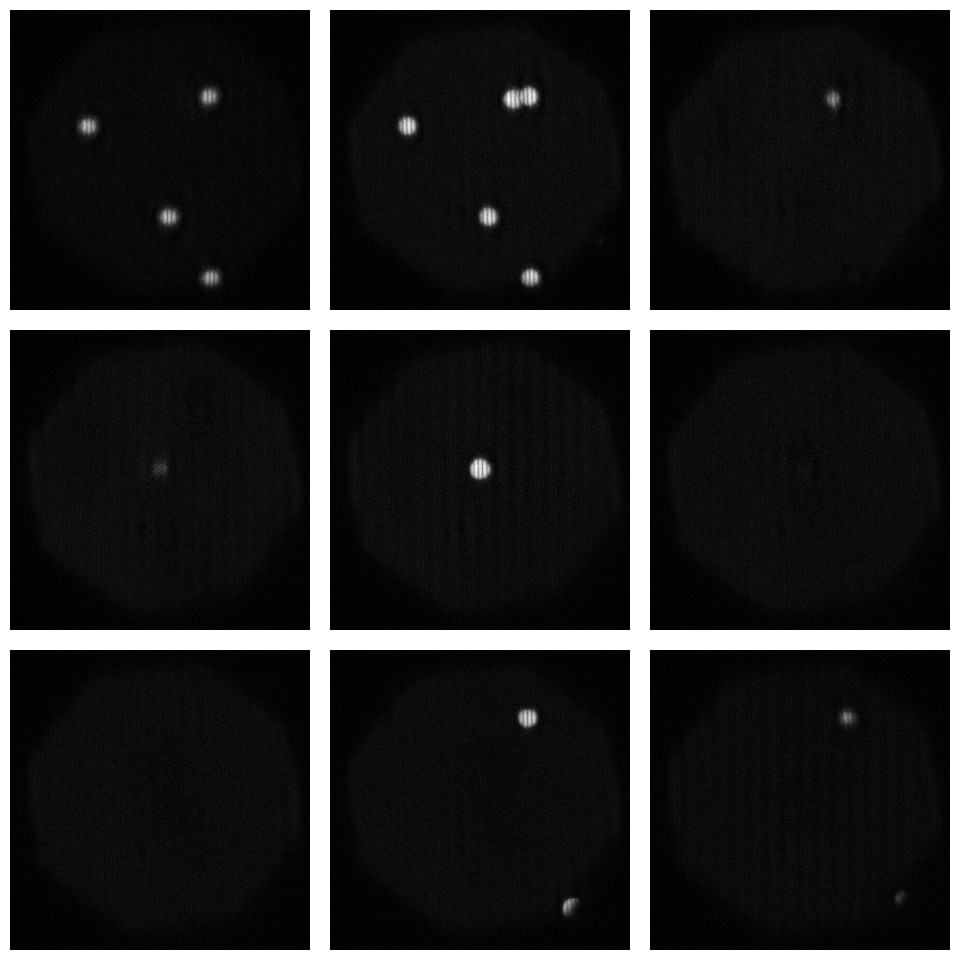
\includegraphics[width=12cm]{m_sec}
  \caption{Computationally sectioned images. Note that two beads (4
    and 7) are very close to the border of the field of view and not
    fully illuminated.}
  \label{fig:m_sec}
\end{figure}

The sectioned images were processed with a three-dimensional
difference-of-Gaussian filter that was matched to enhance the signal
of the beads. Strong local maxima in the result were used as positions
in a sphere model of the sample (see \figref{fig:model}).

\begin{figure}[H]
  \centering
  \includegraphics[width=6cm]{model}
  \caption{Sphere model of the three-dimensional bead distribution
    with bead center positions from \figref{fig:m_sec}.}
  \label{fig:model}
\end{figure}

% bead in wf_004.pgm is  33-12=21 pixels wide, corresponds to 2um
% 25 um diameter of field of view

The coordinates of the beads was then used to selectively illuminate
each by displaying a disk with \unit[3]{$\mu$ m} diameter at the
appropriate position on the LCoS (see \figref{fig:m_clem}). Note that
two beads, that were part in the model, are very dark in these
images. These beads (4 and 7) were very close the border of the field
of view.

\begin{figure}[H]
  \centering
  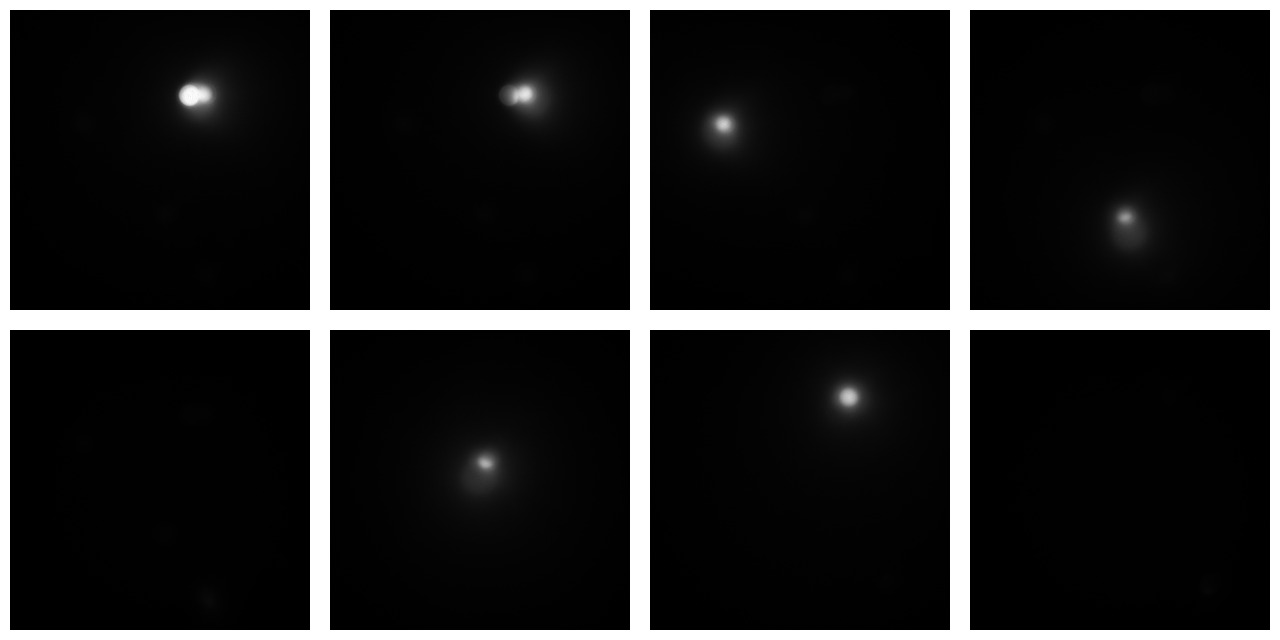
\includegraphics[width=12cm]{m_clem}
  \caption{Spatially controlled illumination of the beads from
    \figref{fig:m_sec}. The top left image shows bead number zero and
    so forth, the second image in the top shows bead number one and so
    on. The MMA is fully white and the LCoS displays a disk at the
    appropriate position to illuminate the target bead. In comparison
    to \figref{fig:m_wf} a strong reduction of out-of-focus
    illumination can be observed.}
  \label{fig:m_clem}
\end{figure}


Finally using the sphere model from \figref{fig:model} we calculated
optimized patterns for the MMA (see also section
\ref{sec:trace-detect}). \figref{fig:m_bfp_img8} shows the results of
raytracing through the model with each bead as a target
nucleus. Bright regions in these images are BFP positions that would
result in ray angles that excite many out-of-focus fluorophores. 

\begin{figure}[H]
  \centering
  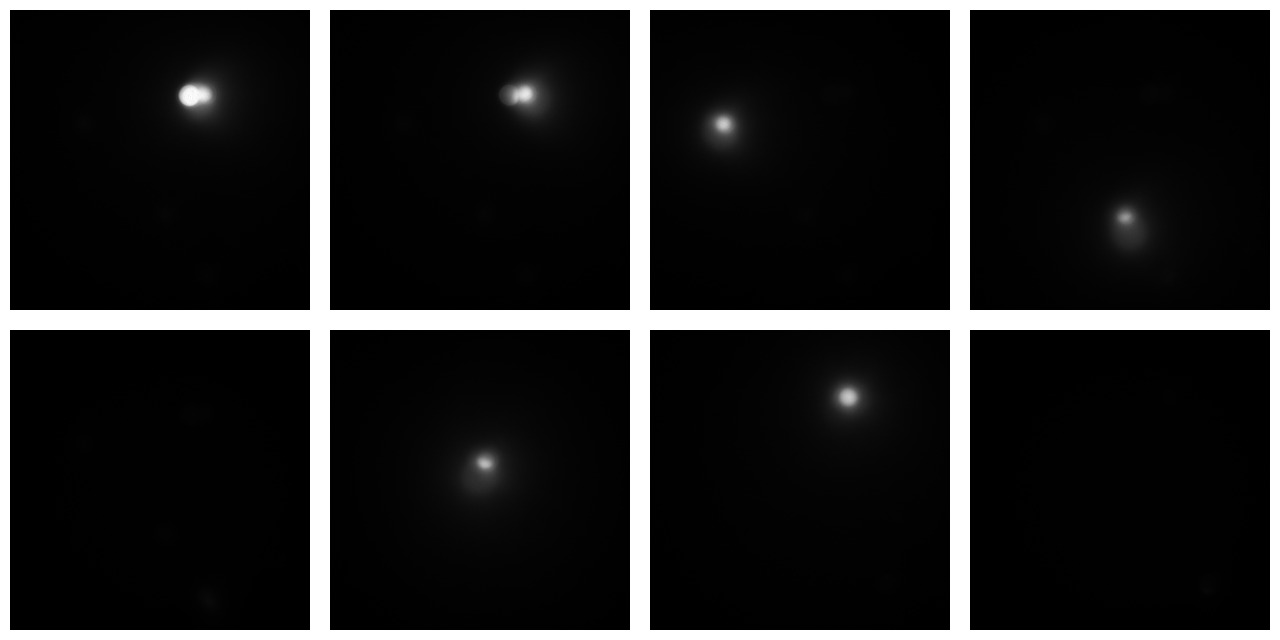
\includegraphics[width=12cm]{m_ang}
  \caption{Spatio-angular controlled illumination of the beads from
    \figref{fig:m_sec}. The top left image shows bead number zero and
    so forth, the second image in the top shows bead number one and so
    on. The LCoS selectively illuminates the target bead and the MMA
    displays the pattern shown in \figref{fig:m_bfp_co}.}
  \label{fig:m_ang}
\end{figure}


In \ref{fig:m_bfp_bw} thresholded masks are shown. The threshold was
chosen such that the darkest quantile of the accumulated shadow maps
in \figref{fig:m_bfp_img8} becomes white. For this particular sample
structure this strategy always led to significant parts of the MMA
being white.

\begin{figure}[H]
  \centering
  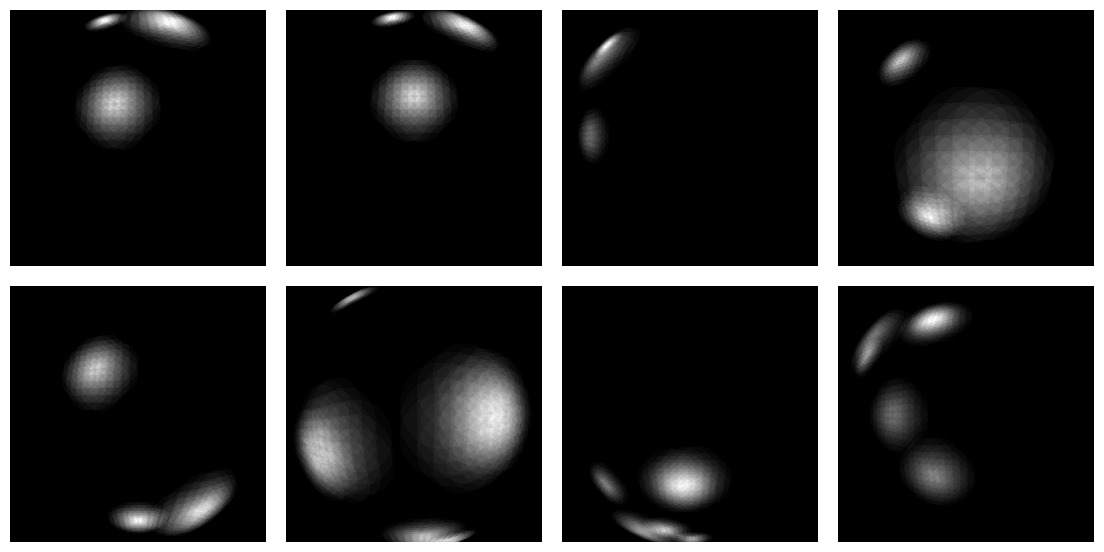
\includegraphics[width=12cm]{m_bfp_img8}
  \caption{Accumulated shadow map (see section \ref{sec:trace-detect})
    obtained by projecting out-of-focus nuclei through several points
    in the target nucleus into the BFP of the objective. Bright areas
    indicate rays that would hit many out-of-focus spheres on their
    way into the target point.}
  \label{fig:m_bfp_img8}
\end{figure}

\begin{figure}[H]
  \centering
  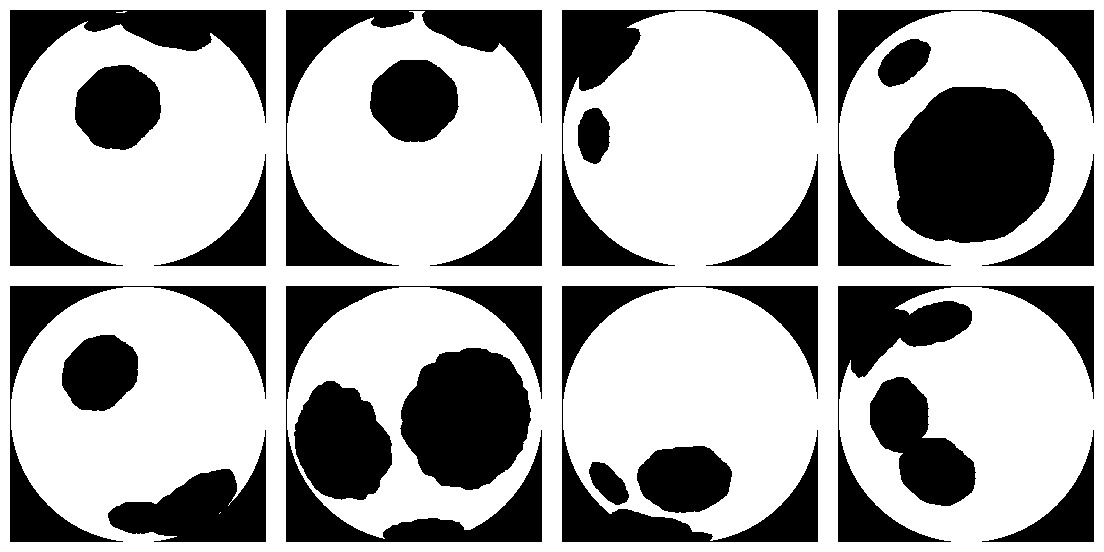
\includegraphics[width=12cm]{m_bfp_bw}
  \caption{Thresholded and inverted version of the accumulated shadow
    maps. The threshold is chosen, so that the darkest quantile of
    \figref{fig:m_bfp_img8} becomes white. The white areas of the
    masks will therefore prevent exposure of out-of-focus
    fluorophores.}
  \label{fig:m_bfp_bw}
\end{figure}

\figref{fig:m_bfp_co} displays a smooth, Gaussian filtered version of
the mask. This pattern was displayed on the MMA while capturing the
images in \figref{fig:m_bfp_co}. The smooth mask is expected to
produce a more uniform light distribution within the sample.


\begin{figure}[H]
  \centering
  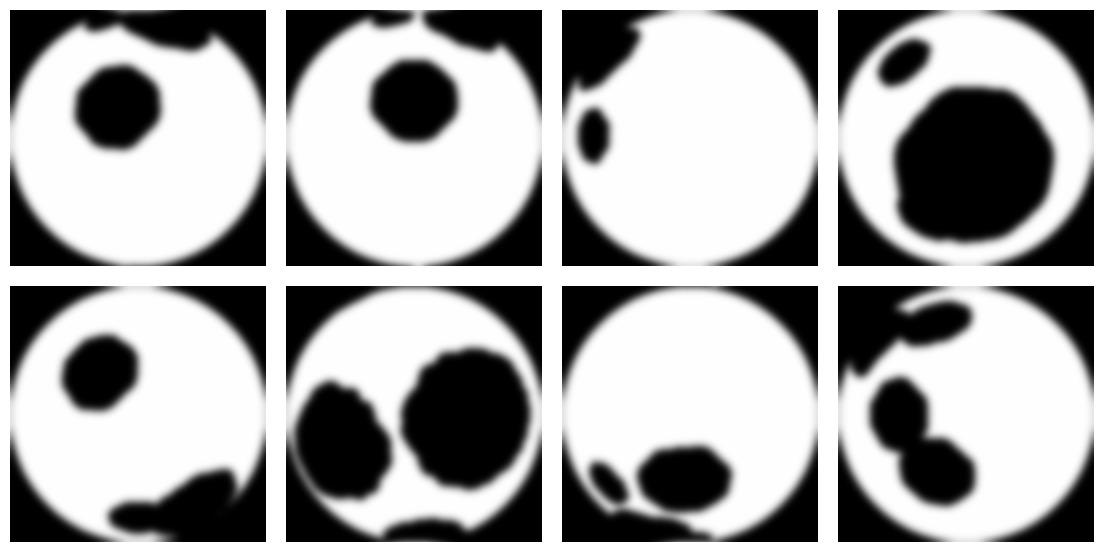
\includegraphics[width=12cm]{m_bfp_co}
  \caption{Smoothed version of the masks from
    \figref{fig:m_bfp_bw}. These were the patterns that were displayed
    on the MMA when the images in \figref{fig:m_ang} were captured.}
  \label{fig:m_bfp_co}
\end{figure}


\begin{figure}[H]
  \centering \subfigure[wide field
  illumination]{\includegraphics[width=3.4cm]{max_wf}}
  \subfigure[optically
  sectioned]{\includegraphics[width=3.4cm]{max_sec}}
  \subfigure[spatial illumination
  control]{\includegraphics[width=3.4cm]{max_clem}}
  \subfigure[spatio-angular illumination
  control]{\includegraphics[width=3.4cm]{max_ang}}
  \caption{Maximum intensity projections of the three-dimensional
    stacks that were obtained with different illumination methods.}
  \label{fig:mip}
\end{figure}

Finally, in \figref{fig:mip} we compare the maximum intensity
projections of the widefield $z-$stack, the sectioned $z-$stack, the
spatially selected beads and the spatio-angular illuminated beads.

Of those the optically sectioned result looks best. However, a lot of
out-of-focus illumination occured, when acquiring this
image. \figref{fig:mip}~c) and d) show what typical images of our
microscope will look like and one can also see some draw backs.

The homogeneous fluorescent background in the embedding medium makes
the spatially illuminated regions visible. However, this would not be
a problem in nuclear tracking problems. For beads 4 and 7 the target
area and illuminated area do not seem to overlap.

\subsection{Conclusion for bead sectioning experiment}
The images with spatial \figref{fig:m_clem} and spatio-angular control
\figref{fig:m_ang} look very much identical. In order to show the
improvement due to angular control more clearly it would have been
useful to have less fluorescence from the embedding medium.

The contrast in the structured illumination images
(\figref{fig:m_phase}) could have been optimized by reducing the
illumination angles with the MMA and ensure that the $\pm
1^\textrm{st}$ orders are not cut off by the pupil of the objective
(see also Appendix \ref{sec:apotome}).

The vertical line artifacts in the computationally reconstructed
optical sections in \figref{fig:m_phase} only occured with laser
illumination and not with LED illumination. In this experiment the
artifacts do not influence the localization precision of the beads.
However, we investigated other reconstruction algorithms in Appendix
\ref{sec:app_hilo} which don't show these artifacts and can also work
with only one patterned image and one uniform image.

